\section{Bode-Diagramm}

Das Bode-Diagramm ist eine weitere Variante, den Frequenzgang $G(\jimg \omega)$ grafisch darzustellen.
Die Darstellung beinhaltet zwei Graphen.

\begin{itemize}
    \item Amplitudengang $|G(\jimg \omega)|$ in Dezibel $\deci \bel$
    \item Phasengang $\angle G(\jimg \omega)$ in Grad $\degree$
    \item Die Frequenzachse ist \textbf{logarithmisch} mit $\log_{10}(\omega)$
    \item \textbf{Ein Bodediagramm kann in ein Nyquistdiagramm umgezeichnet werden, aber nicht umgekehrt!}
\end{itemize}


% Bei zu wenig Platz weglassen
\subsubsection{Logarithmische Frequenzachse}{134}

\begin{outline}
    \1 Serieschaltung von Systemen
        $$ G(\jimg \omega) = G_1(\jimg \omega) \cdot G_2(\jimg \omega) $$

        \2 Amplitudengang
            $$ |G(\jimg \omega)| = |G_1(\jimg \omega)| \cdot |G_2(\jimg \omega)| $$
            $$ |G(\jimg \omega)|_{\deci \bel} = |G_1(\jimg \omega)|_{\deci \bel} + |G_2(\jimg \omega)|_{\deci \bel} $$
            \textrightarrow\ Grafisch multiplizieren wäre schwierig, grafisch addieren geht gut

        \2 Phasengang
            $$ \angle G(\jimg \omega) = \angle G_1(\jimg \omega) +  \angle G_2(\jimg \omega) $$
            \textrightarrow\ Die Phase muss nicht logarithmisch sein, wir haben schon eine Addition 
\end{outline}


\subsection{Vorgehen: Bode-Diagramm zeichnen}
\label{Bodediagramm zeichnen}

Das Diagramm wird approximativ mit \textbf{Geraden} gezeichnet!

\begin{outline}
    \1 Frequenzgang in folgende Form bringen:
        $$ G(\jimg \omega) = K_0 \cdot (\jimg \omega)^v \cdot \frac{(1 + T_{n0} \cdot \jimg \omega)\cdot (1 + T_{n1} \cdot \jimg \omega) \cdot \ldots}
        {(1 + T_{p0} \cdot \jimg \omega)\cdot (1 + T_{p1} \cdot \jimg \omega) \cdot \ldots} \cdot e^{- \jimg \omega T_t} $$
        \2 Für $\omega = 0$ sind alle $(1 + T \cdot \jimg \omega) = 1 = 0 \, \deci \bel$
        \2 Für $\omega = \frac{1}{T}$ sind alle  $(1 + T \cdot \jimg \omega) = 1 + \jimg = \sqrt{2} \cdot e^{\jimg \frac{\pi}{4}} 
            = 3 \, \deci \bel \angle 45 \, \degree$
    \1 Frequenzen der Nullstellen berechnen: $\omega = \frac{1}{T_n}$
    \1 Frequenzen der Polstellen berechnen: $\omega = \frac{1}{T_p}$


    \1 Jede \textbf{Nullstelle} bewirkt
        \2 einen Knick um $+ 20 \, \deci \bel$ / Dekade \textbf{nach oben} im Amplitudengang
        \2 einen Phasenhub von $+ 90 \, \degree$ über 2 Dekaden \textrightarrow\ $+ 45 \, \degree$ beim Knick
    \1 Jede \textbf{Polstelle} bewirkt
        \2 einen Knick um $- 20 \, \deci \bel$ / Dekade \textbf{nach unten} im Amplitudengang
        \2 einen Phasenverlust von $- 90 \, \degree$ über 2 Dekaden \textrightarrow\ $- 45 \, \degree$ beim Knick
    \1 Einzelne Faktoren einzeichnen \textrightarrow\ Wenn Faktor quadriert ist, zwei mal einzeichnen!
    \1 Grafische Addition der Faktoren für gesamten Frequenzgang
\end{outline}


\example{Bode-Diagramm zeichnen}
\vspace{-0.2cm}
$$ G(\jimg \omega) = \frac{\jimg \omega + 10}{(\jimg \omega + 0.1)} \quad  \underrightarrow{\text{ Standardform }} \quad 
  G(\jimg \omega) = \cgn{100} \cdot \frac{(\cvt{1 + 0.1 \, \jimg \omega})}{(\cbl{ 1 + 10 \, \jimg \omega})} $$

  \begin{itemize}
    \item $ \cgn{\abs{K_0}_{\deci \bel} = \abs{100}_{\deci \bel} = 40 \, \deci \bel}$ \textrightarrow\ $\angle G(100) = 0 \, \degree$
    \item Nullstelle: \cvt{$\abs{1 + 0.1 \, \jimg \omega}_{\deci \bel}$} \textrightarrow\ Knick bei $\omega = \frac{1}{0.1 \, \second} = 10 \frac{\rad}{\second}$
    \item Polstelle: \cbl{$\abs{1 + 10 \, \jimg \omega}_{\deci \bel}$} \textrightarrow\ Knick bei $\omega = \frac{1}{10 \, \second} = 0.1 \frac{\rad}{\second}$
    \item \cor{Endresultat}: Grafische Addition der Teilresultate
  \end{itemize}

\begin{center}
    % Gain
    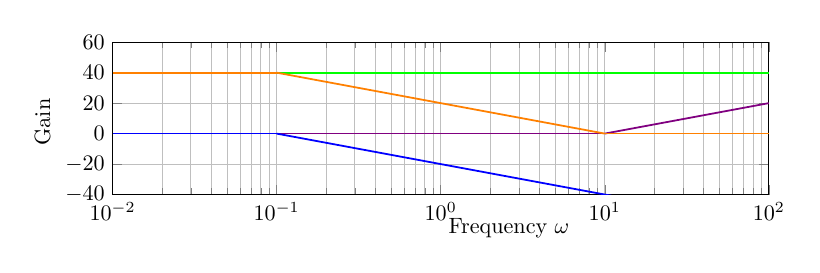
\begin{tikzpicture}
        [
            scale = 0.8,
            >=latex
        ]
        \begin{axis}
            [
                width=12cm,
                height=4cm,
                xmode=log,
                xmin=0.01, xmax=100, ymin=-40, ymax=60,
                x label style={anchor=west},
                xlabel=Frequency $\omega$,
                y label style={anchor=south},
                ylabel=Gain $\deci \bel$,
                xmajorgrids=true,
                xminorgrids=true,
                ymajorgrids=true
            ]
            
            % K_0
            \addplot[thick, color=green, domain=0.01:100]{40};

            % Nullstelle
            \addplot[thick, color=violet, domain=0.01:10]{0};               % start bis Knick
            \addplot[thick, color=violet, domain=10:100]{20*log10(x)-20};   % ab Knick nach oben    

            % Polstelle
            \addplot[thick, color=blue, domain=0.01:0.1]{0};                % start bis Knick
            \addplot[thick, color=blue, domain=0.1:100]{-20*log10(x)-20};   % ab Knick nach oben    
            
            % Grafische Addition
            \addplot[thick, color=orange, domain=0.01:0.1]{40};    
            \addplot[thick, color=orange, domain=0.1:10]{-20*log10(x)+20};        
            \addplot[thick, color=orange, domain=10:100]{0};      
           
        \end{axis}
        
    \end{tikzpicture}

    \vspace{0.3cm}


    % Phase
    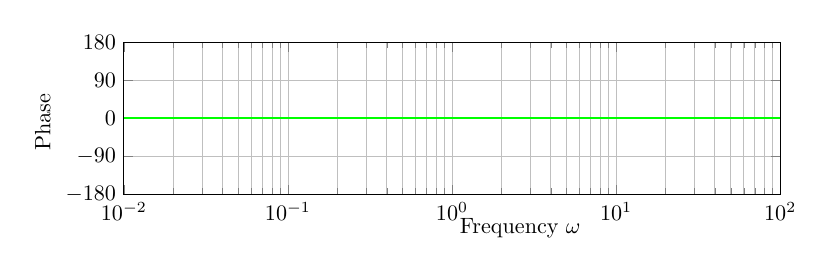
\begin{tikzpicture}
        [
            scale = 0.8,
            >=latex
        ]
        \begin{axis}
            [
                width=12cm,
                height=4cm,
                xmode=log,
                xmin=0.01, xmax=100, ymin=-180, ymax=180,
                x label style={anchor=west},
                xlabel=Frequency $\omega$,
                y label style={anchor=south},
                ylabel=Phase $\degree$,
                ytick={-180, -90, 0, 90, 180},
                % yticklabels={-180, -90, 0, 90, 180},
                xmajorgrids=true,
                xminorgrids=true,
                ymajorgrids=true
            ]
            
            % K_0
            \addplot[thick, color=green, domain=0.01:100]{0};
                
            % Nullstelle
            % \addplot[thick, color=violet, domain=0.01:1]{0};              % start bis Knick
            % \addplot[thick, color=violet, domain=1:10]{};        % ab Knick nach oben    
            
            % Polstelle
            % \addplot[thick, color=blue, domain=0.01:0.1]{0};                % start bis Knick
            % \addplot[thick, color=blue, domain=0.1:100]{-20*log10(x)-20};   % ab Knick nach oben    
            
            % Grafische Addition
            % \addplot[thick, color=orange, domain=0.01:0.1]{40};    
            % \addplot[thick, color=orange, domain=0.1:10]{-20*log10(x)+20};        
            % \addplot[thick, color=orange, domain=10:100]{0};      


            
        \end{axis}
            
    \end{tikzpicture}
\end{center}


\subsubsection{Inverse Frequenzgänge}{137}

Um das Bodediagramm des inversen Frequenzgangs $\frac{1}{G(\jimg \omega)}$ zu erhalten, muss bei Betrag \textbf{und} Phase
das \textbf{Vorzeichen gedreht} werden.
\vspace{0.2cm}
 
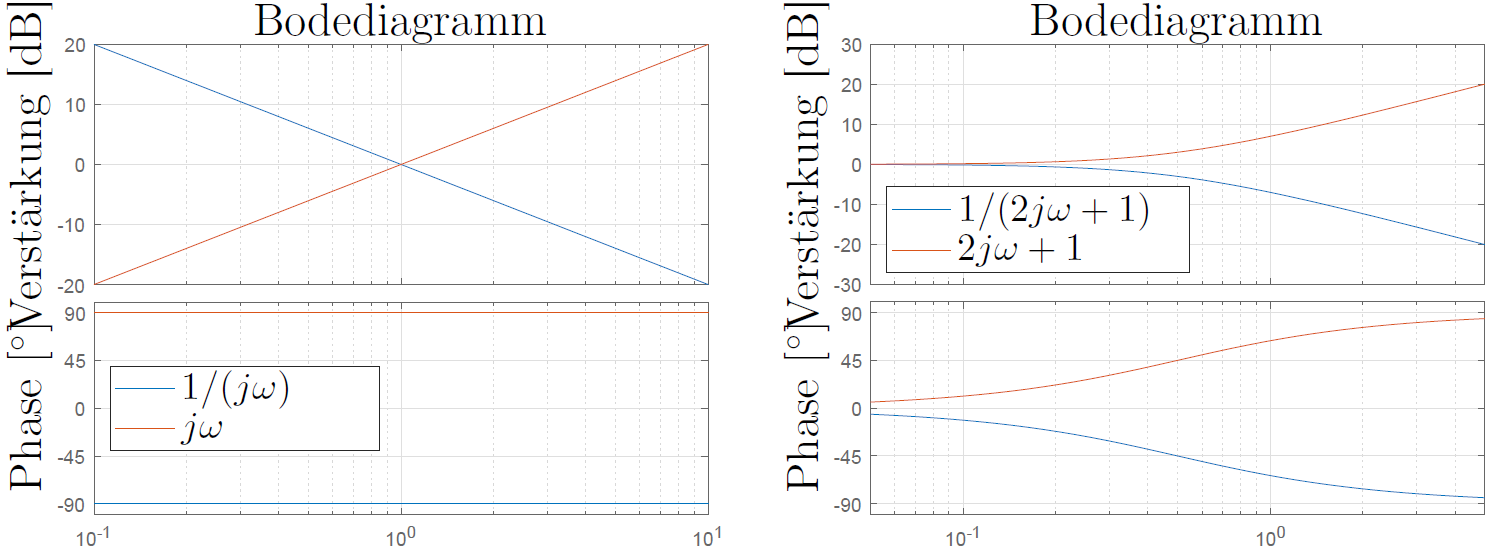
\includegraphics[width=\columnwidth]{images/inverse_frequenzgaenge.png}


\subsubsection{Lead-Lag-Glied}
\label{Lead-Lag-Glied}

$$ \boxed{ \text{Lead-Lag-Glied: } \quad G(s) = K \cdot \frac{s T_1 + 1}{s T_2 + 1} } $$

\begin{minipage}[c]{0.48\columnwidth}
    \begin{center}
        \myul{Lead-Glied ($T_1 > T_2$)}
    \end{center}
    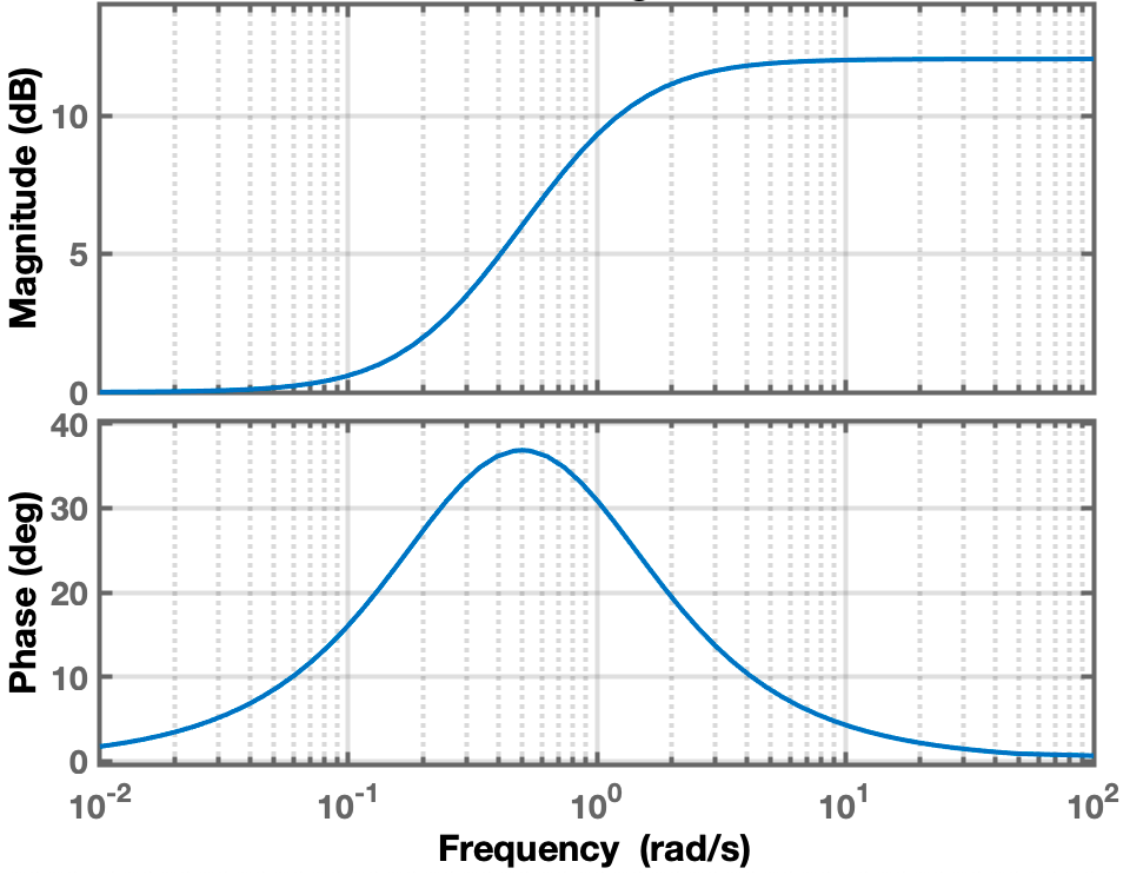
\includegraphics[width=\columnwidth]{images/bode_lead-glied.png}
\end{minipage}
\hfill
\begin{minipage}[c]{0.48\columnwidth}
    \begin{center}
        \myul{Lag-Glied ($T_2 > T_1$)}
    \end{center}
    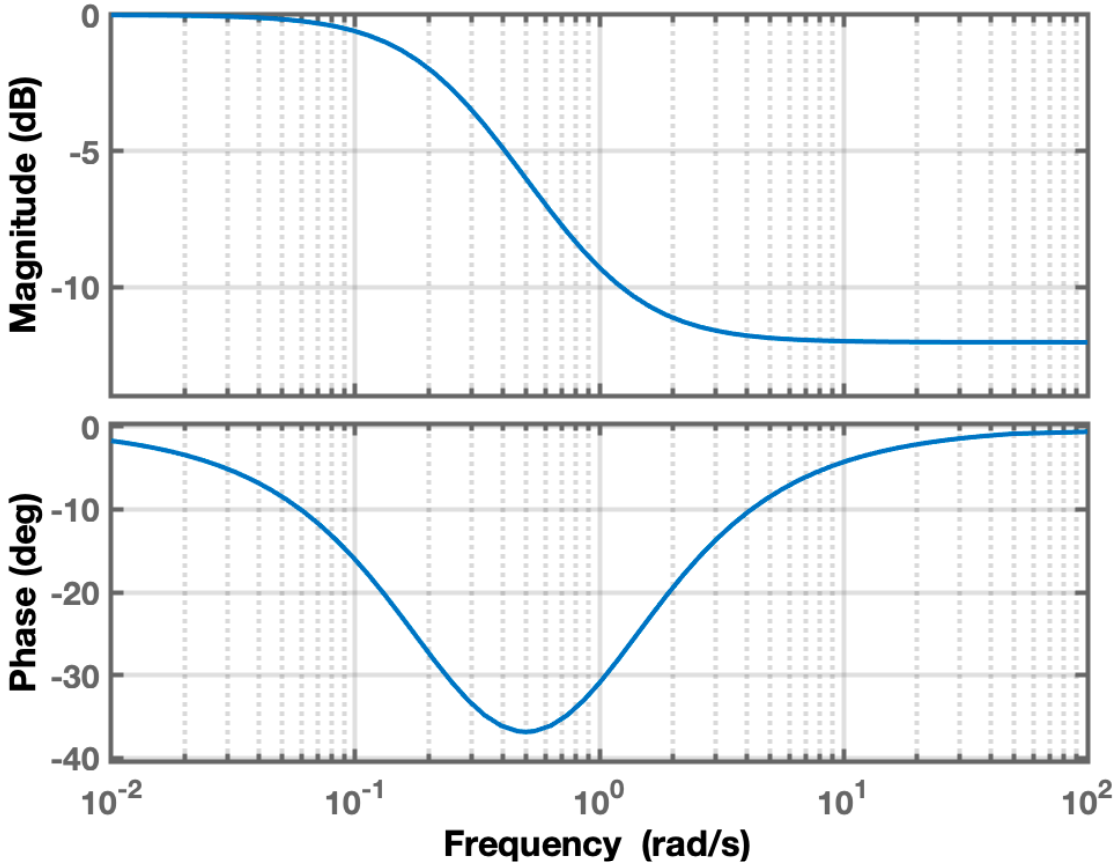
\includegraphics[width=\columnwidth]{images/bode_lag_glied.png}
\end{minipage}

$$ \boxed{ \text{Maximale Phasenänderung bei:} \quad \omega = \frac{1}{\sqrt{T_1 \cdot T_2}} } $$
\textrightarrow\ Bei der Regler-Auslegung werden vor allem Lead-Glieder verwendet, um \textbf{Phase anheben} zu können


\subsection{Modellbildung (UTF) mittels Frequenzmessung}{139}

Um aus einem gegebenen Bodediagramm die Übertragungsfuntion $G(\jimg \omega)$ zu ermitteln, werden die Zeichenregeln aus Abschnitt
~\ref{Bodediagramm zeichnen} \textbf{rückwärts angewendet}. Dazu werden die Punkte einer gegebenen Messung mittels Geraden approximiert.
Mittels dieser Approximationen können die einzelen Komponenten (Faktoren) der gesuchten UTF ermittelt werden.


\example{Übertragungsfuntion $G(s)$ aus Bodediagramm ermitteln}

\begin{minipage}[c]{0.5\columnwidth}
    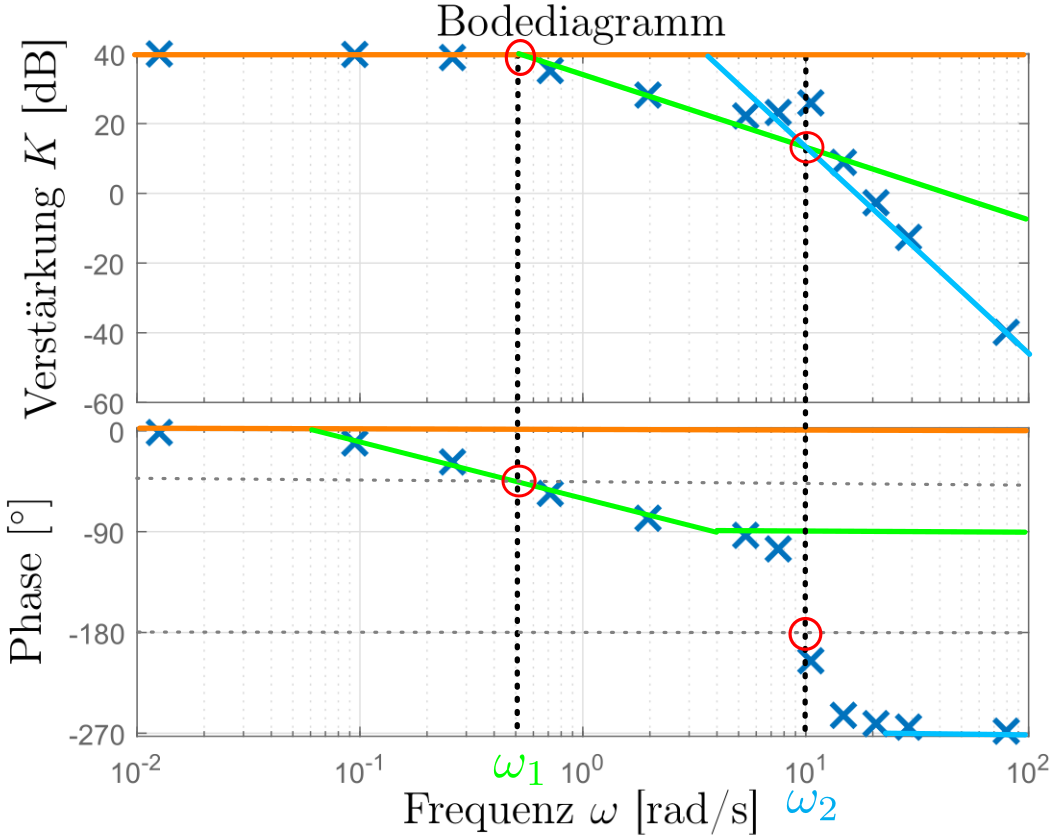
\includegraphics[width=\columnwidth]{images/bode_zu_modell.png}
\end{minipage}
\hfill
\begin{minipage}[c]{0.48\columnwidth}
    Aus den Steigungen der Geraden ist ersichtlich, dass folgende Komponenten in $G(s)$ enthalten sein müssen: \\
    \cor{Verstärkung $K$}, \cgn{$\text{PT}_1$-Glied}, \textcolor{cyan}{$\text{PT}_2$-Glied}
    $$ G(s) = \cor{K} \cdot \cgn{\frac{1}{(s T_1 + 1)}} \cdot \textcolor{cyan}{\frac{1}{(T_2^2 s^2 + 2 \zeta T_2 s + 1)}} $$
    Werte der Parameter aus Bodediagramm bestimmen:
    \begin{itemize}
        \item \cor{$|K|_{\deci \bel} = 40$ \textrightarrow\ $K = 100$}
        \item \cgn{$\omega_1 = \frac{1}{T_1} = 0.5$ \textrightarrow\ $T_1 = \frac{1}{0.5} = 2$}
        \item \textcolor{cyan}{$\omega_2 = \frac{1}{T_2} = 10$ \textrightarrow\ $T_1 = \frac{1}{10} = 0.1$}
        \item \textcolor{cyan}{$\zeta = 0.1$} \textrightarrow\ gegeben 
    \end{itemize}
\end{minipage}



\subsection{Stabilität im Bodediagramm}{140}
Analog zum Punkt $-1$ im Nyquistdiagramm kann die Stabilität auch im Bodediagramm beurteilt werden. Auch bei dieser Betrachtung 
sind die folgenden Frequenzen relevant.

\begin{itemize}
    \item Durchtrittsfrequenz $\omega_{D}$ \textrightarrow\ Phasenreserve $\Phi_{\rm RES}$ \\
        Frequenz, bei der die Verstärkung 1 ist: $| G_{0}(\jimg \omega_{D})| = 1 \, (= 0 \, \deci \bel)$
    \item Phasenschnittfrequenz $\omega_{\pi}$ \textrightarrow\ Verstärkungsreserve $\Phi_{\rm RES}$ \\
        Frequenz, bei der die Phase $-180 \, \degree$ beträgt: $\angle {G_{0}(\jimg \omega_{\pi})} = - \pi \, \rad \, (= -180 \, \degree)$
\end{itemize}


\subsubsection[Parameter K_{\rm RES} und  \Phi_{\rm RES} aus Bodediagramm lesen]{Parameter $K_{\rm RES}$ und  $\Phi_{\rm RES}$ aus Bodediagramm lesen}

\begin{minipage}[c]{0.55\columnwidth}
    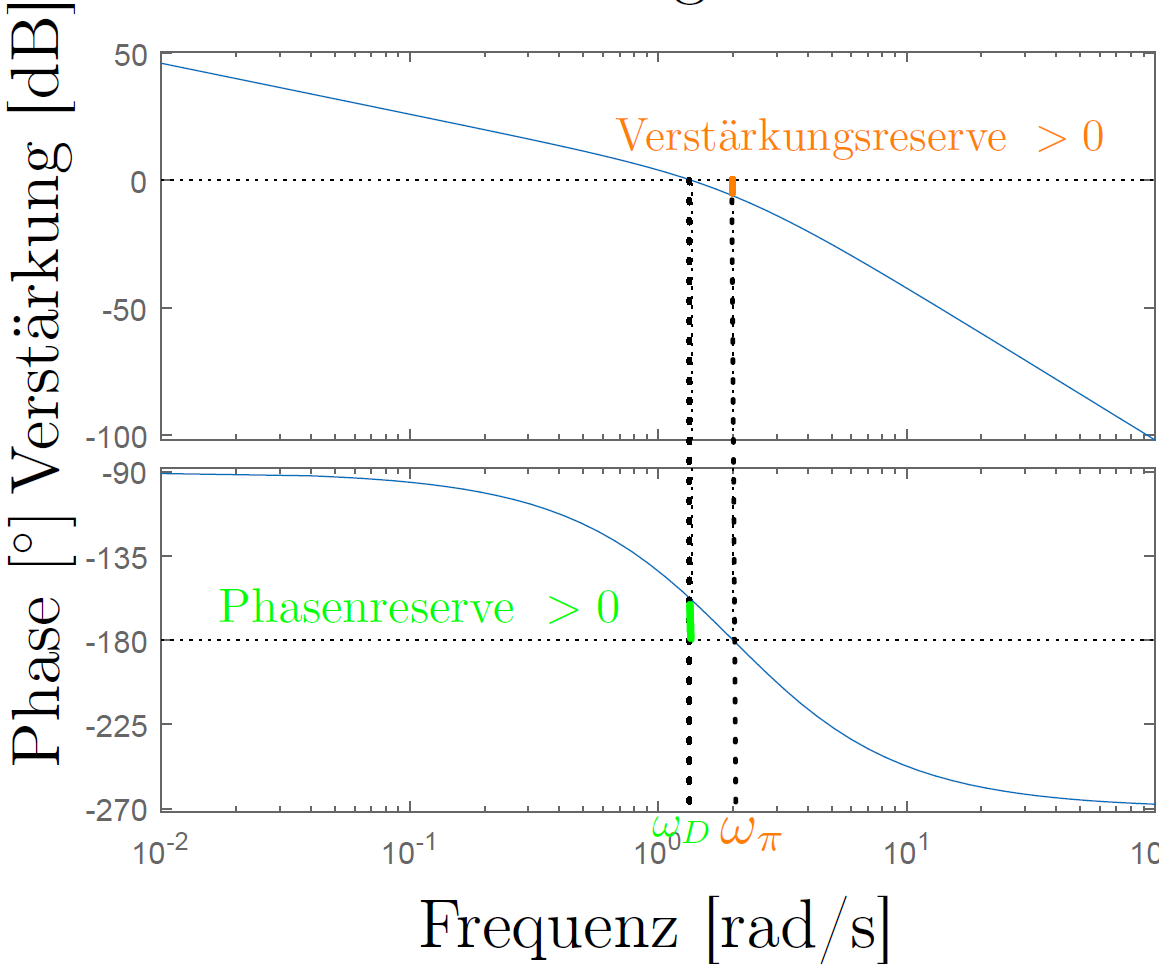
\includegraphics[width=\columnwidth]{images/bodeplot_stabilitaetsreserven.png}
\end{minipage}
\hfill
\begin{minipage}[c]{0.42\columnwidth}
    \raggedright%
    \begin{itemize}
        \item \cgn{Durchtrittsfrequenz $\omega_{D}$} 
            $$ K_{\rm RES} = 0 \, \deci \bel - K_{\text{@} 180 \degree } $$ 

        \item \cor{Phasenschnittfrequenz $\omega_{\pi}$} 
            $$ \Phi_{\rm RES} = \Phi_{\text{@}0 \deci \bel }  + 180 \, \degree $$ 
    \end{itemize}
    \crd{\textbf{Achtung:} Das Vorzeichen von $\Phi_{\rm RES}$ bzw. $\Phi_{\rm RES}$ ist essentiell für die Stabilitäts-Beurteilung und
    darf auf keine Fall vernachlässigt werden!}
\end{minipage}


\subsubsection{Beurteilung der Stabilität des Systems}

Wenn das System die \textbf{Anforderungen des Nyquist-Kriteriums erfüllt}, verhält sich die Stabilität des Systems folgendermassen:

\begin{itemize}
    \item \textbf{Grenzstabilität}: Amplitudengang bei $0 \, \deci \bel$ \textbf{und} Phasengang bei $-180 \, \degree$
    \item \textbf{Instabilität}:  $K_{\rm RES} < 0$ \textbf{und} $\Phi_{\rm RES} < 0$ (ergibt sich automatisch, wenn einer der 
        beiden Parameter $< 0$ ist)
    \item \textbf{Stabilität}: $K_{\rm RES} > 0$ \textbf{und} $\Phi_{\rm RES} > 0$ 
    \item \textbf{Stabilität}: $\omega_{\pi} > \omega_D$  % gemäss Skript
\end{itemize}


\subsection{Bodediagramme mit Matlab}

\lstinputlisting{snippets/bode.m}


\subsection{Alternative Stabilitätskriterien -- Vorzeichenregel}{142}

Die Stabilität kann alternativ 'direkt' au sden Parametern der \textbf{Differentialgleichung} (des
Frequenzgangs) des \textbf{geschlossenen Regelkreises} bestimmt werden.\\
Aus der DGL der Form
$$ \sum\limits_{k=0}^n a_k \cdot y^{(k)}(t) = \sum\limits_{k=0}^m b_k \cdot u^{(k)}(t) $$
kann das \textbf{charakteristische Polynom} ermittelt werden. Daraus kann dann mittels 
folgender \textbf{Vorzeichenregel} eine Aussage über die Stabilität des \textbf{geschlossenen Regelkreises} 
gemacht werden.

\fbox{\parbox{0.95\columnwidth}{
Eine \textbf{notwendige} Stabilitätsbedingung für das \cbl{charakteristische Polynom}
$$ \cbl{a_n \lambda^n + a_{n-1} \lambda_{n-1} + \ldots + a_2 \lambda^2  + a_1 \lambda + a_0 } $$
besteht darin, das alle Koeffizienten existieren $a_0 \ldots a_n$ (also $\neq 0$ sind) \textbf{und dasselbe Vorzeichen} haben. \\
Bei System erster und zweiter Ordnung ist die Vorzeichenregel auch \textbf{hinreichend} für die Stabilität.
}}


\example{Stabil, instabil oder 'keine Ahnung'}

\begin{minipage}{0.3\columnwidth}
    \begin{center}
        \textbf{stabil}
    \end{center}
    $$ \frac{1}{\cbl{s^2 + 5s + 7}} $$
\end{minipage}
\hfill
\begin{minipage}{0.3\columnwidth}
    \begin{center}
        \textbf{instabil}
    \end{center}
    $$ \frac{1}{\cbl{s^2 -7s + 3}} $$
\end{minipage}
\hfill
\begin{minipage}{0.3\columnwidth}
    \begin{center}
        \textbf{keine Ahnung}
    \end{center}
    $$ \frac{1}{\cbl{s^3 + 2 s^2 + s + 4}} $$
\end{minipage}


\example{Stabilität aus geschlossenem Regelkreises bestimmen}

\begin{minipage}[c]{0.56\columnwidth}
    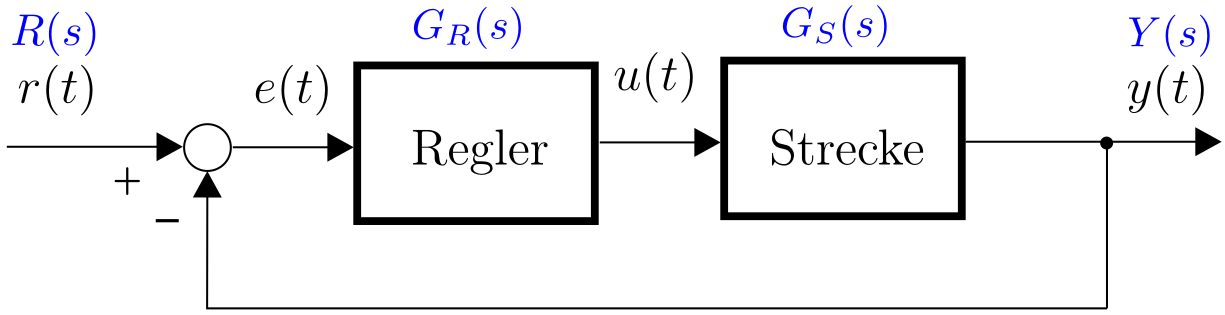
\includegraphics[width=\columnwidth]{images/beispiel_regelkreis_vorzeichenkriterium.png}
\end{minipage}
\hfill
\begin{minipage}[c]{0.42\columnwidth}
    \begin{center}
        UTF geschlossener Regelkreis: 
    \end{center}
    $$ \boxed{ T(s) = \frac{Y(s)}{R(s)} = \frac{G_R(s) \cdot G_S(s)}{1 + G_R(s) \cdot G_S(s)} } $$
\end{minipage}

\vspace{0.2cm}
$G_R(s)$ und $G_S(s)$ seien gegeben als: $G_R(s) = K_R, \quad  G_S(s) =\frac{K}{s(sT + 1)} = \frac{K}{T s^2 + s} $
$$ \Rightarrow  T(s) = \frac{G_R(s) \cdot G_S(s)}{1 + G_R(s) \cdot G_S(s)} 
= \frac{\frac{K_R \cdot K}{T s^2 + s}}{1 + \frac{K_R \cdot K}{T s^2 + s}} 
= \frac{K_R \cdot K}{\cbl{T s^2 + s + K_R \cdot K}} \text{\textrightarrow\ stabil für } K_R, K, T > 0 $$

